
\documentclass[xcolor={usenames,dvipsnames},12pt,presentation,aspectratio=169]{beamer}

\usepackage[utf8]{inputenc}
\usepackage{fontawesome}
\usepackage[brazilian]{babel}
\usepackage{verbatim}
\usepackage{graphicx}
\usepackage{xspace}
\usepackage{amsthm}
\usepackage{url}
\usepackage{array}
\usepackage{hyperref}
\usepackage{times,mathptmx}
\usepackage{pdfpages}
\usepackage{mdframed}
\usepackage{tikz}
\usepackage{alltt}
\usepackage{minted}
%\usepackage{times}
%\usepackage[usenames,dvipsnames]{xcolor}
%\usepackage[usenames,dvipsnames]{color}
%\usepackage{color}

\usetikzlibrary{arrows,shapes}

\usetheme{Madrid}
%\usetheme{Boadilla}
%\usetheme{Darmstadt}
%\usetheme{Frankfurt}
%\usetheme{CambridgeUS}
%\usetheme{AnnArbor}
%\usecolortheme{beaver}
%\usecolortheme{seahorse}
%\usecolortheme{seagull}
\usecolortheme[named=BrickRed]{structure}

\setbeamercovered{transparent}

\setbeamertemplate{footline}[frame number]
%\setbeamertemplate{navigation symbols}{}
%\setbeamersize{text margin left=1em,text margin right=1em}

\newcommand{\titulo}{Avaliação de Desempenho}
\newcommand{\disciplina}{ELC139 - Programação Paralela}
\newcommand{\nome}{João Vicente Ferreira Lima (UFSM)}

\lecture[1]{\aula}{aula01}
\def\lecturename{\aula}

\newcommand{\Red}[1]{{\color{red}#1}}
\newcommand{\red}[1]{{\color{red}#1}}
\newcommand{\Blue}[1]{{\color{blue}#1}}
\newcommand{\blue}[1]{{\color{blue}#1}}

\newcommand{\PBS}[1]{\let\temp=\\#1\let\\=\temp}
\newcommand{\RRCOL}{\PBS\raggedright\hspace{0pt}}

\newcommand{\p}[1]{\texttt{#1}}
\newenvironment{code}{%
  \begin{alltt}%
  }{%
  \end{alltt}%
}

\makeatletter
%\setbeamertemplate{headline}{}
% {%
%   \leavevmode%
%   \@tempdimb=2.4375ex%
%   \ifnum\beamer@subsectionmax<\beamer@sectionmax%
%     \multiply\@tempdimb by 4%
%   \else%
%     \multiply\@tempdimb by\beamer@subsectionmax%
%   \fi%
%   \ifdim\@tempdimb>0pt%
%     \advance\@tempdimb by 1.125ex%
%     \begin{beamercolorbox}[wd=.5\paperwidth,ht=\@tempdimb]{section in head/foot}%
%       \vbox to\@tempdimb{\vfil\insertsectionnavigation{.5\paperwidth}\vfil}%
%     \end{beamercolorbox}%
%     \begin{beamercolorbox}[wd=.45\paperwidth,ht=\@tempdimb]{subsection in head/foot}%
%       \vbox
%       to\@tempdimb{\vfil\insertsubsectionnavigation{.45\paperwidth}\vfil}%
%     \end{beamercolorbox}%
%     \begin{beamercolorbox}[wd=.05\paperwidth,ht=\@tempdimb]{subsection in head/foot}%
%       \vbox
%       to\@tempdimb{\vfil\hfil\insertframenumber\vfil\vfil}%
%     \end{beamercolorbox}%
%   \fi%
% }

\def\dohead{\beamer@headcounter=4\relax\beamer@headcounter=1\loop\ifnum\beamer@headcounter<\beamer@totalheads%
  \advance\beamer@headcounter by1\relax%
  \csname @@head\the\beamer@headcounter\endcsname\repeat}

\makeatother

\title[\titulo]{\titulo}

\subtitle{\disciplina}

\author[João V. F. Lima]{\nome}

%\institute[UFSM]{Departamento de Linguagens e Sistemas de Computação \\ Universidade Federal de Santa Maria \\ \url{jvlima@inf.ufsm.br} \\ \url{http://www.inf.ufsm.br/~jvlima}}
\institute[UFSM]{Universidade Federal de Santa Maria \\ \url{jvlima@inf.ufsm.br} \\ \url{http://www.inf.ufsm.br/~jvlima}}
\date{2023/1}

\graphicspath{{.}{figs/}}

\logo{ 
\includegraphics[height=1.5cm,width=1.5cm,keepaspectratio]{logo_inf}    
        
\includegraphics[height=1.5cm,width=1.5cm,keepaspectratio]{logo_ufsm} }

%\titlegraphic{
%	
\includegraphics[width=2cm]{logo_ufsm}
%  \hspace{1cm}
%	
\includegraphics[width=2cm]{logo_inf}
%}

\newtheorem{mydef}{Definição}[section]
%\newtheorem{myteo}{Teorema}[section]
%------------------------------------------------------------------------------
%\newcommand{\xkaapi}{XKaapi\xspace}
%------------------------------------------------------------------------------
% Typesetting Listings
\usepackage{listings}
\lstset{
  language=C,
  %basicstyle=\scriptsize\ttfamily,
  %basicstyle=\normalsize\ttfamily,
  basicstyle=\small\ttfamily,
  %basicstyle=\footnotesize\ttfamily,
  %aboveskip=0pt,
  %belowskip=0pt,
  %mathescape=false,
  columns=fullflexible,
  %numbers=none,
  numbers=left,
  numbersep=5pt,
%  showtabs=true,
%  showspaces=true,
  frame=tb,
  breaklines=true
}
%------------------------------------------------------------------------------
%\lstset{commentstyle=\color{blue}}
%\lstset{stringstyle=\ttfamily}
%\lstset{ classoffset=1, 
%            morekeywords={kaapi,omp,task,data,alloca, declare, reduction, identity, parallel,sync,taskwait,cilk,spawn,tbb,css,cilk\_spawn,cilk\_sync,cilk\_for,offload},
%            keywordstyle=\color{Red}\bfseries
%           }
%\lstset{ classoffset=2, 
%            morekeywords={value,read,write,readwrite,reduction,untied,firstprivate,TaskBodyCPU,TaskBodyGPU,ka,Signature,RW,CW,range2d\_r,range2d\_rw,range2d,Spawn,Fork,Shared\_w,Shared\_r,Shared,a1,target,device,copyin,copyout,input,implements,copy\_deps,RPWP,range2d\_rpwp,rangeindex,Memory,Register,SetStaticSched,Sync,Unregister,Community,System,join\_community,SpawnMain,leave,initialize,terminate,logfile,array,SetArch,ArchHost,ArchCUDA,W,R,gpuStream,pointer\_w,pointer\_r,pointer\_cw,pointer},
%            keywordstyle=\color{Blue}\bfseries
%           }
%\lstset{ classoffset=3, 
%            morekeywords={storage,ld},
%            keywordstyle=\bfseries
%           }
%\lstset{ classoffset=4, 
%            morekeywords={in,out,inout,cout,concurrent},
%            keywordstyle=\color{Red}\bfseries
%           }
%           
%\lstset{classoffset=0, showstringspaces=false}
%------------------------------------------------------------------------------
\mdfsetup{
  backgroundcolor=gray!10,
%  roundcorner=10pt,
}
%------------------------------------------------------------------------------
\newcommand{\restorefootline}{\setbeamertemplate{navigation symbols}{}}
%\newcommand{\setfootline}[1]{\setbeamertemplate{navigation symbols}{\textcolor{black}{\textbf{#1}}}}
\newcommand{\includeslides}[4]{%
%  \setfootline{#1}%
  {
    \setbeamercolor{background canvas}{bg=}
    \includepdf[pages={#1},%
    pagecommand={},
%    pagecommand={\begin{frame}[default]{}\end{frame}},
%    #4,%
    turn=false,noautoscale=false,column=false,columnstrict=false,openright=false,frame=false]{#2}%
  }
  %\restorefootline%
}
%------------------------------------------------------------------------------
\begin{document}

\begin{frame}
%  \titlepage
  \maketitle
%  \mode<presentation>
%  {
%    \begin{columns}
%      \begin{column}{0.5\textwidth}
%      \raggedleft
%	
\includegraphics[width=2cm]{logo_ufsm}
%      \end{column}
%      \begin{column}{0.5\textwidth}
%	
\includegraphics[width=2cm]{logo_inf}
%      \end{column}
%    \end{columns}
%  }
\end{frame}

\begin{frame}
    \frametitle{Outline}
    \tableofcontents[hideallsubsections]
%    \tableofcontents
\end{frame}

\AtBeginSection{
  \begin{frame}
    \frametitle{Outline}
    \tableofcontents[currentsection,hideothersubsections]
  \end{frame}
}


%%%%%%%%%%%%%%%%%%%%%%%%%%%%%%%%%%%%%%%%%%%%%%%%%%%%%%%%%%%%%%%%%%%%%%%%%%%%%%
\section{Métricas de Desempenho}
%%%%%%%%%%%%%%%%%%%%%%%%%%%%%%%%%%%%%%%%%%%%%%%%%%%%%%%%%%%%%%%%%%%%%%%%%%%%%%%
%------------------------------------------------------------------------------
\begin{frame}[fragile]
  \frametitle{Speedup}
\begin{itemize}
  \item Número de processadores/cores $= p$
  \item Tempo de execução sequencial $= T_{serial}$
  \item Tempo de execução paralelo em $p$ processadores $= T_p$
  \item Speedup $= S$
\end{itemize}
  \begin{equation*}
    S = \frac{T_{serial}}{T_{p}}
  \end{equation*}
  \begin{center}
    Se $T_p = \frac{T_{serial}}{p} \rightarrow$ \textbf{speedup linear}
  \end{center}
\end{frame}
%------------------------------------------------------------------------------
\begin{frame}[fragile]
  \frametitle{Eficiência}
  \begin{center}
    \begin{equation*}
      E = \frac{S}{p} = \frac{\frac{T_{serial}}{T_p}}{p} = \frac{T_{serial}}{p * T_p}
    \end{equation*}
  \end{center}
   \begin{center}
 	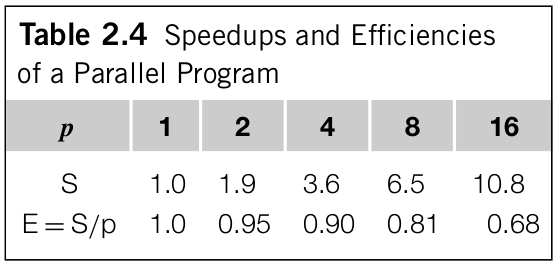
\includegraphics[width=0.6\textwidth]{speedup1.png}
   \end{center}
   \vfill
   {\tiny Introduction to Parallel Computing, Grama et al, 2003.}
\end{frame}
%------------------------------------------------------------------------------
\begin{frame}[fragile]
  \frametitle{Eficiência}
   \begin{center}
 	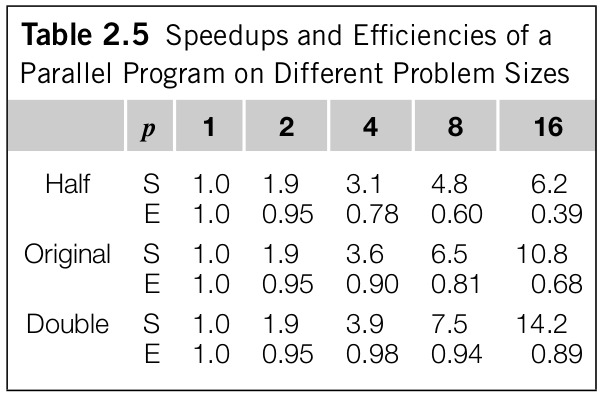
\includegraphics[width=0.6\textwidth]{speedup2.png}
   \end{center}
   \vfill
   {\tiny Introduction to Parallel Computing, Grama et al, 2003.}
\end{frame}
%------------------------------------------------------------------------------
\begin{frame}[fragile]
  \frametitle{Speedup}
  \vspace{-3mm}
   \begin{center}
 	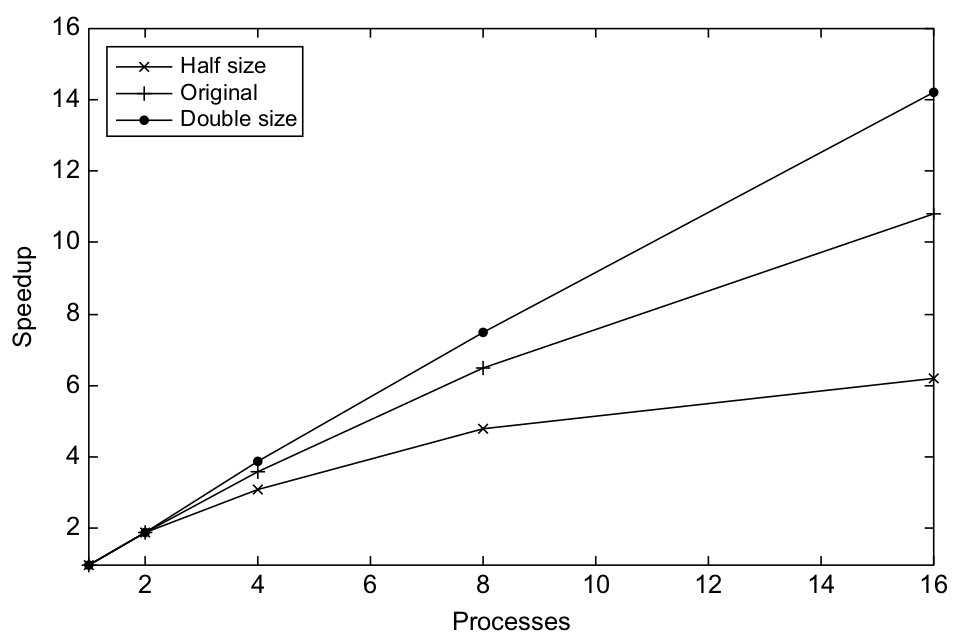
\includegraphics[width=0.7\textwidth]{speedup3.png}
   \end{center}
   \vfill
   {\tiny Introduction to Parallel Computing, Grama et al, 2003.}
\end{frame}
%------------------------------------------------------------------------------
\begin{frame}[fragile]
  \frametitle{Eficiência}
  \vspace{-3mm}
   \begin{center}
 	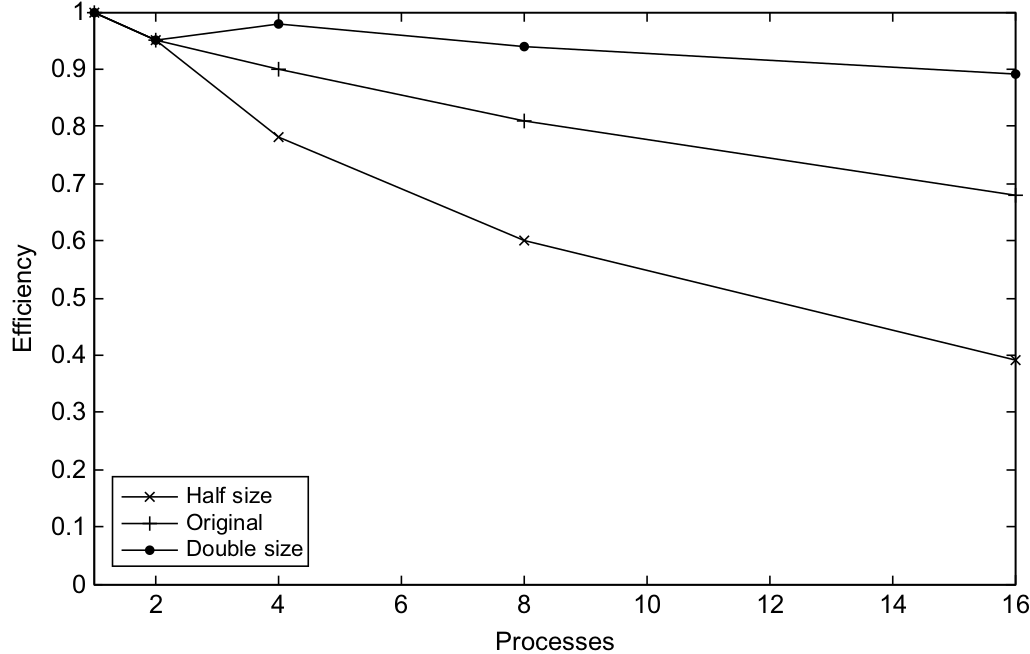
\includegraphics[width=0.71\textwidth]{speedup4.png}
   \end{center}
   \vfill
   {\tiny Introduction to Parallel Computing, Grama et al, 2003.}
\end{frame}
%------------------------------------------------------------------------------
\begin{frame}[fragile]
  \frametitle{Speedup}
  \vspace{-3mm}
   \begin{center}
 	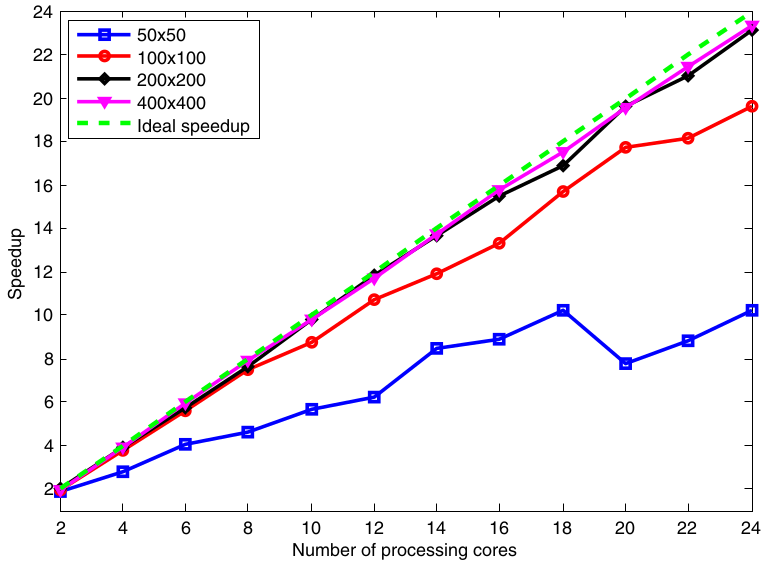
\includegraphics[width=0.6\textwidth]{artigo1.png}
   \end{center}
   %\vfill
   \vspace{-5mm}
   {\tiny On the parallel efficiency and scalability of the correntropy coefficient for image analysis. 
   https://doi.org/10.1186/s13173-014-0018-4}
\end{frame}
%------------------------------------------------------------------------------
\begin{frame}[fragile]
  \frametitle{Sobrecusto}
\begin{itemize}
  \item Speedup/eficiência aumenta com o tamanho do problema
  \item Muitos programas paralelos adicionam um sobrecusto (\emph{overhead}) de dividir o trabalho
\end{itemize}
  \begin{equation*}
    T_p = \frac{T_{serial}}{p} + T_{overhead}
  \end{equation*}
\begin{itemize}
  \item Uma das formas de medir o sobrecusto paralelo é medindo o tempo do
    programa paralelo com um processador $T_1$
\end{itemize}
  \begin{equation*}
    T_{overhead} = \frac{T_{1}}{T_{serial}}
  \end{equation*}
\end{frame}
%------------------------------------------------------------------------------
\begin{frame}[fragile]
  \frametitle{Speedup}
  \begin{block}{Tempo sequencial $T_{serial}$}
    \begin{itemize}
      \item Qual implementação sequencial?
      \item Versão base da paralela ou outra versão?
    \end{itemize}
  \end{block}
\begin{itemize}
  \item Exemplo: shell sort paralelo
  \begin{itemize}
    \item Shell sort sequencial?
    \item $T_1$?
    \item Quicksort?
    \item Mesmo processador ou outro mais rápido?
  \end{itemize}
\end{itemize}
\end{frame}
%%%%%%%%%%%%%%%%%%%%%%%%%%%%%%%%%%%%%%%%%%%%%%%%%%%%%%%%%%%%%%%%%%%%%%%%%%%%%%
\section{Leis de Amdahl e Gustafson}
%%%%%%%%%%%%%%%%%%%%%%%%%%%%%%%%%%%%%%%%%%%%%%%%%%%%%%%%%%%%%%%%%%%%%%%%%%%%%%%
%------------------------------------------------------------------------------
\begin{frame}[fragile]
  \frametitle{Lei de Amdahl}
\begin{itemize}
  \item Observação feita por Gene Amdahl em 1960, mais tarde \textbf{Lei de Amdahl}
    \item O speedup máximo é limitado independentemente do número de processadores, 
  a menos que a totalidade do programa seja paralelo
  \begin{itemize}
    \item Speedup máximo de $\frac{1}{r}$ onde $r$ é a fração não paralela
  \end{itemize}
\end{itemize}
\begin{exampleblock}{Exemplo}
\begin{itemize}
  \item 90\% do programa é paralelo e $T_{serial} = 20$. Então:
\end{itemize}
\vspace{2mm}
$T_p = 0.9 * \frac{T_{serial}}{p} + 0.1 * T_{serial}  = 18/p + 2$

\vspace{2mm}
$S = \frac{T_{serial}}{0.9 * T_{serial} + 0.1 * T_{serial}}  = \frac{20}{18/p + 2}$

\vspace{2mm}
Se $p \rightarrow \infty$ então $S <= \frac{T_{serial}}{0.1 * T_{serial}} = \frac{20}{10} = 10$
\end{exampleblock}
\end{frame}
%------------------------------------------------------------------------------
\begin{frame}[fragile]
  \frametitle{Lei de Gustafson}
  Há diversas razões para não se preocupar com a lei de Amdahl. Quanto maior o problema menor a parte sequencial na maioria dos problemas.
\begin{itemize}
  \item Muitos problemas apresentam speedup significativos em sistemas distribuídos.
  \item Speedup pequeno não é problema, sobretudo quando o esfoço é pequeno.
\end{itemize}
\end{frame}
%------------------------------------------------------------------------------
\begin{frame}[fragile]
  \frametitle{Escalabilidade}
  O problema é escalável se a  eficiência $E$ permaneçe constante quando aumentamos o tamanho do problema e o número de processadores.

  Se é \textbf{escalável} podemos tratar problemas maiores.
\begin{itemize}
  \item \textbf{Escalabilidade forte} -- a eficiência é mantida se $p$ cresce sem aumentar o tamanho do problema.
  \item \textbf{Escalabilidade fraca} -- a eficiência é mantida se $p$ cresce e também aumenta o tamanho do problema.
\end{itemize}
\end{frame}
%%%%%%%%%%%%%%%%%%%%%%%%%%%%%%%%%%%%%%%%%%%%%%%%%%%%%%%%%%%%%%%%%%%%%%%%%%%%%%
\section{Medindo tempo}
%%%%%%%%%%%%%%%%%%%%%%%%%%%%%%%%%%%%%%%%%%%%%%%%%%%%%%%%%%%%%%%%%%%%%%%%%%%%%%%
%------------------------------------------------------------------------------
\begin{frame}[fragile]
  \frametitle{Medindo tempo}
  \begin{itemize}
  \item Como medir o tempo ?
  \begin{itemize}
    \item Tempo de processamento
    \item Tempo de E/s
    \item Tempo de comunicação
    \item Tempo de barreira  (\emph{wall clock time})
  \end{itemize}  
  \item Não estamos interessados no tempo entre começo e fim do programa no geral.
  \begin{itemize}
    \item Em um bubble sort, estamos interessados no tempo para ordenar as chaves.
    \item Não queremos o tempo para ler ou imprimir as chaves.
  \end{itemize}  
  \item Queremos o tempo entre quando o primeiro processo começou a execução do código até quando o último processo terminou a execução.
\end{itemize}
\end{frame}
%------------------------------------------------------------------------------
\begin{frame}[fragile]
  \frametitle{Medindo tempo}
  \begin{itemize}
    \item Função hipotética que retorna o tempo em segundos desde um tempo fixo.
    \begin{itemize}
      \item UNIX é 01/01/1970
    \end{itemize}
    \item As APIs tem uma função de tempo.
    \begin{itemize}
      \item \mintinline{C}{MPI_Wtime}
      \item \mintinline{C}{omp_get_wtime}
    \end{itemize}
  \end{itemize}
\begin{center}
\begin{minipage}{0.9\textwidth}
  \begin{minted}[linenos, frame=lines]{C}
double start, finish;

start = Get_current_time();

/* Code that we want to time */

finish = Get_current_time();
printf("The elapsed time = %e seconds\n", finish-start);
  \end{minted}
\end{minipage}
\end{center}  
\end{frame}
%------------------------------------------------------------------------------
\begin{frame}[fragile]
  \frametitle{Medindo tempo}
  \begin{itemize}
    \item A sincronização pode ser garantida por barreiras.
  \end{itemize}
\begin{center}
\begin{minipage}{0.9\textwidth}
  \begin{minted}[linenos, frame=lines]{C}
double global_elapsed ;
double my_start , my_finish , my_elapsed;
/* Synchronize all processes/threads */
Barrier ();
my_start = Get_current_time ();
/* Code that we want to time */
my_finish = Get_current_time ();
my_elapsed = my_finish - my_start ;
/* Find the max across all processes/threads */
global_elapsed = Global_max ( my_elapsed );
if ( my_rank == 0)
  printf ("The elapsed time = %e seconds\n", global_elapsed );
  \end{minted}
\end{minipage}
\end{center}  
\end{frame}
%------------------------------------------------------------------------------
\begin{frame}[fragile]
  \frametitle{Medindo tempo}
  \vspace{-4mm}  
  \begin{columns}
      \begin{column}{0.3\textwidth}
        Como apresentar os tempos?
        \begin{itemize}
          \item Média -- $\mu$
          \item Mediana 
          \item Desvio padrão -- $\sigma$
          \item Intervalo de confiança
        \end{itemize}    
      \end{column}
      \begin{column}{0.7\textwidth}
        \begin{center}
          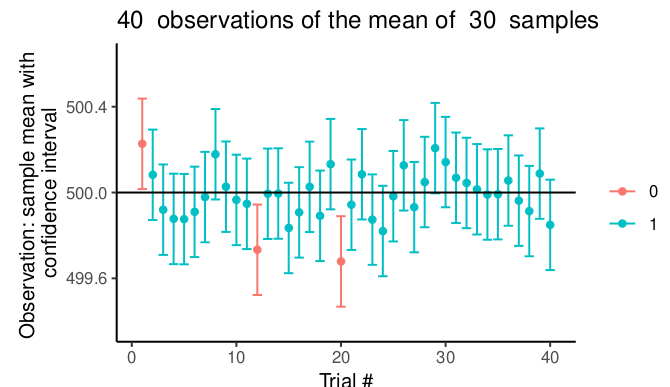
\includegraphics[width=0.9\textwidth]{CI_illustration.png}
          \end{center}       
          \vspace{-3mm}  
          \begin{block}{Intervalo de confiança}
            Chance de 95\% da média real estar dentro de $2\frac{\sigma}{\sqrt{n}}$ da média da amostra.
          \end{block}
          %\textbf{Intervalo de confiança} -- Chance de 95\% da média real estar dentro de $2\frac{\sigma}{\sqrt{n}}$ da média da amostra.
      \end{column}
    \end{columns}
\end{frame}
%------------------------------------------------------------------------------
\begin{frame}[fragile]
  \frametitle{Medindo tempo}
  \begin{itemize}
    \item Assumindo que temos duas alternativas $A$ e $B$ 
    \item Temos as médias $\mu_{A}$ e $\mu_{B}$ e intervalos de confiança
    \item Os dois intervalos de confiança com 95\% não sobrepõem
  \end{itemize}
  \begin{columns}
    \begin{column}{0.4\textwidth}
    Então $\mu_A < \mu_B$ com 95\% de confiança.
    \end{column}
    \begin{column}{0.6\textwidth}
      \begin{center}
        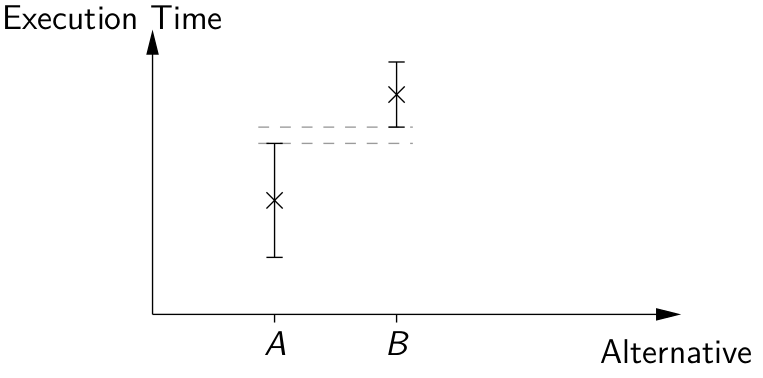
\includegraphics[width=\textwidth]{ci1.png}
     \end{center}           
    \end{column}
  \end{columns}
\end{frame}
%------------------------------------------------------------------------------
\begin{frame}[fragile]
  \frametitle{Medindo tempo}
  \begin{itemize}
    \item Assumindo que temos duas alternativas $A$ e $B$ 
    \item Temos as médias $\mu_{A}$ e $\mu_{B}$ e intervalos de confiança
    \item Os dois intervalos de confiança com 95\% se sobrepõem.
  \end{itemize}
  \begin{columns}
    \begin{column}{0.4\textwidth}
    \textbf{Nada podemos concluir!!}
    \end{column}
    \begin{column}{0.6\textwidth}
      \begin{center}
        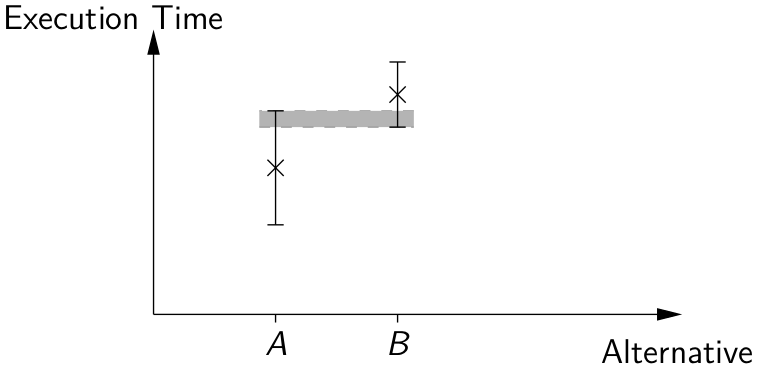
\includegraphics[width=\textwidth]{ci2.png}
     \end{center}           
    \end{column}
  \end{columns}
\end{frame}
%------------------------------------------------------------------------------
\begin{frame}[fragile]
  \frametitle{Medindo tempo}
  \begin{itemize}
    \item Assumindo que temos duas alternativas $A$ e $B$ 
    \item Temos as médias $\mu_{A}$ e $\mu_{B}$ e intervalos de confiança
    \item Os dois intervalos de confiança com 95\% se sobrepõem.
  \end{itemize}
  \begin{columns}
    \begin{column}{0.4\textwidth}
    \textbf{Nada podemos concluir!!}
    \end{column}
    \begin{column}{0.6\textwidth}
      \begin{center}
        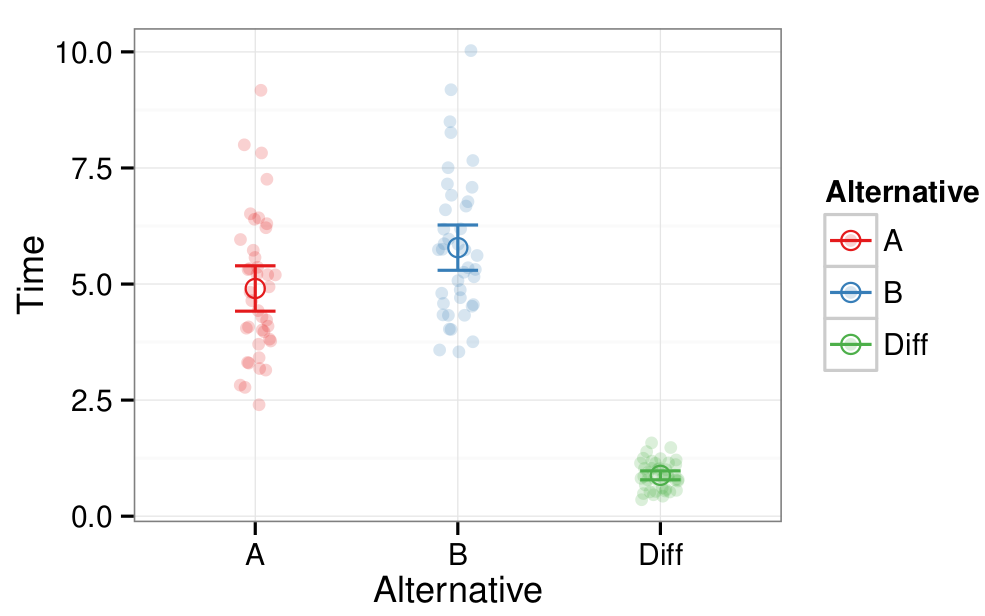
\includegraphics[width=\textwidth]{ci3.png}
     \end{center}           
    \end{column}
  \end{columns}
\end{frame}
%------------------------------------------------------------------------------
%------------------------------------------------------------------------------
\begin{frame}[plain]{}
  \begin{center}
    \vspace{2cm}
    \Large{https://joao-ufsm.github.io/par2023a/}
    
    \vspace{1cm}
    
\includegraphics[width=2cm]{logo_ufsm}
    \hspace{0.5cm}
    
\includegraphics[width=2cm]{logo_inf}
  \end{center}
\end{frame}
%------------------------------------------------------------------------------

\end{document}
